\documentclass[11pt, a4paper]{article}
\usepackage[utf8]{inputenc}
\usepackage{amsmath,setspace,geometry}
\usepackage{amsfonts}
\usepackage[shortlabels]{enumitem}
\usepackage{rotating}
\usepackage{pdflscape}
\usepackage{graphicx}
\usepackage{bbm}
\usepackage[dvipsnames]{xcolor}
\usepackage[colorlinks=true, linkcolor= BrickRed, citecolor = BrickRed, filecolor = BrickRed, urlcolor = BrickRed, hypertexnames = true]{hyperref}
\usepackage[]{natbib} 
\bibpunct[:]{(}{)}{,}{a}{}{,}
\geometry{left = 1.0in,right = 1.0in,top = 1.0in,bottom = 1.0in}
\usepackage[english]{babel}
\usepackage{float}
\usepackage{subfig}
\usepackage{booktabs}
\usepackage{pdfpages}
\usepackage{threeparttable}
\usepackage{lscape}
\usepackage{bm}
\setstretch{1.4}
%\usepackage[tablesfirst,nolists]{endfloat}


\newtheorem{theorem}{Theorem}
\newtheorem{assumption}{Assumption}
\newtheorem{lemma}{Lemma}
\newtheorem{definition}{Definition}
\newtheorem{proposition}{Proposition}
\newtheorem{claim}{Claim}
\newtheorem{corollary}{Corollary}
\newtheorem{example}{Example}

\title{Revisiting Conduct Parameter Estimation in Homogeneous Goods Markets: At Least, Linear Model is Valid}
\author{Yuri Matsumura\footnote{Department of Economics, Rice University. Matsumura: \texttt{\href{mailto:Yuri.Matsumura@rice.edu}{Yuri.Matsumura@rice.edu}}} \and Suguru Otani \footnote{Department of Economics, Rice University. Otani: \texttt{\href{mailto:so19@rice.edu}{so19@rice.edu}}}}

\begin{document}

\maketitle

\begin{abstract}
    We revisit the conduct parameter estimation in homogeneous goods markets. In contrast to the pessimistic simulation results of linear models shown in \cite{perloff2012collinearity}, our simulation shows that the estimation becomes accurate by properly adding demand shifters in the supply estimation and increasing the sample size. We also investigate log-linear models widely used in Industrial Organization literature and recommended by \cite{perloff2012collinearity} and find other estimation problems. Based on the numerical investigation, at least the linear model can achieve a proper estimation of the conduct parameter.
\end{abstract}
% 84words

\section{Introduction}

Measuring competitiveness is one of the important tasks in Empirical Industrial Organization literature.
Conduct parameter is regarded as a useful measure of competitiveness. 
However, it cannot be measured directly from data because data usually lack information about marginal cost.
Therefore, the researchers have tried to identify and estimate the conduct parameter.

The literature has considered two popular specifications of the model for conduct parameter estimation in homogeneous good markets; one is the model with linear demand and marginal cost and the other is the model with log-linear demand and marginal cost.

As for the linear model, \citet{bresnahan1982oligopoly} considers the identification of conduct parameter. 
\citet{perloff2012collinearity} (hereafter, PS) theoretically show that the model is suffering from the multicollinearity problem when the error terms in the demand and supply equations are zero and show by simulations that the parameters cannot be estimated accurately even when the error terms are not zero.
To avoid the problems, the paper recommends using log-linear or some other functional form for at least one of the equations.
As for the log-linear model, the identification strategy is provided by \citet{lau1982identifying}. 
The specification is often used in empirical papers such as \cite{okazaki2022excess} and \cite{merel2009measuring}.

We find the following problems.
As for the linear model, the simulation in PS lacks an excluded demand shifter in the supply equation estimation. 
Also, the paper does not check the effect of increasing the sample size. 
As for the log-linear model, to the best of our knowledge, there is no simulation study to justify the claim of PS.

Given these problems, we revisit the estimation of the conduct parameter in homogeneous product markets.
We confirm that the accuracy of the estimation holds by including a demand shifter in the supply equation estimation properly. 
When the sample size is more than 100, the accuracy of the estimation is also improved.

Next, we examine the log-linear model and numerically show that standard regression estimates an incorrect conduct parameter because the specification adds another estimation problem.
Thus, we conclude that the linear model is a valid specification for the conduct parameter estimation in homogeneous good markets.

% 366 words by Suguru


\section{Model}
The researcher has data with $T$ markets with homogeneous products.
Assume that there are $N$ firms in each market.
Let $t = 1,\ldots, T$ be the index of markets.
Then, we obtain the supply equation:
\begin{align}
     P_t = -\theta\frac{\partial P_t(Q_t)}{\partial Q_t}Q_t + MC_t(Q_t),\label{eq:supply_equation}
\end{align}
where $Q_t$ is the aggregate quantity, $P_t(Q_{t})$ the demand function, $MC_{t}(Q_{t})$ the marginal cost function, and $\theta\in[0,1]$ which is called conduct parameter. 
The equation nests perfect competition, $\theta=0$, Cournot competition, $\theta=1/N, N$ firm symmetric perfect collusion, $\theta=1$, etc.\footnote{See \cite{bresnahan1982oligopoly}.} 

Consider an econometric model of the above model.
Assume that the demand function and the marginal cost function are written as: 
\begin{align}
    P_t = f(Q_t, Y_t, \varepsilon^{d}_{t}, \alpha) \label{eq:demand}\\
    MC_t = g(Q_t, W_{t}, \varepsilon^{c}_{t}, \gamma)\label{eq:marginal_cost}
\end{align}
where $Y_t$ and $W_{t}$ are the vector of exogenous variables, $\varepsilon^{d}_{t}$ and $\varepsilon^{c}_{t}$ the error terms, and $\alpha$ and $\gamma$ are the vector of parameters.
We also have the demand-side and supply-side instrument variables $Z^{d}_{t}$ and $Z^{c}_{t}$ and assume that the error terms satisfy the mean independence condition $E[\varepsilon^{d}_{t}\mid Y_t, Z^{d}_{t}] = E[\varepsilon^{c}_{t} \mid W_{t}, Z^{c}_{t}] =0$.

%254 words by Suguru

\section{Identification of the conduct parameter}

\subsection{Linear demand and linear cost}
Assume that linear demand and cost functions are specified as:
\begin{align}
    P_t &= \alpha_0 - (\alpha_1 + \alpha_2Z^{R}_{t})Q_t + \alpha_3 Y_t + \varepsilon^{d}_{t},\label{eq:linear_demand}\\
    MC_t &= \gamma_0  + \gamma_1 Q_{t} + \gamma_2 W_{t} + \gamma_3 R_t + \varepsilon^{c}_{t},\label{eq:linear_marginal_cost}
\end{align}
where $W_{t}$ and $R_t$ are excluded cost shifter. Equation \eqref{eq:supply_equation} is written as:
\begin{align}
    P_t = \gamma_0 + [\theta(\alpha_1 + \alpha_2Z^{R}_{t})+ \gamma_1] Q_t   + \gamma_2 W_{t} + \gamma_3 R_t + \varepsilon^{c}_{t}.\label{eq:linear_supply_equation}
\end{align}
By substituting Equation \eqref{eq:linear_demand} into Equation \eqref{eq:linear_supply_equation} and solving it for $P_t$, we can represent the aggregate quantity $Q_t$ based on the parameters and exogenous variables as:
\begin{align*}
    Q_t =  \frac{\alpha_0 + \alpha_3 Y_t - \gamma_0 - \gamma_2 W_{t} - \gamma_3 R_t + \varepsilon^{d}_{t} - \varepsilon^{c}_{t}}{(1 + \theta) (\alpha_1 + \alpha_2 Z^{R}_{t}) + \gamma_1}.
\end{align*}


\subsection{Log-linear demand and log-linear marginal cost}

Assume that log-linear demand and cost functions are specified as:
\begin{align}
    \log P_{t} &= \alpha_0 - (\alpha_1 + \alpha_2 Z^{R}_{t}) \log Q_t + \alpha_3 \log Y_t + \varepsilon^{d}_{t},\label{eq:log_linear_demand}\\
    \log MC_t &= \gamma_0 + \gamma_1 \log Q_t +  \gamma_2 \log W_{t} + \gamma_3 \log R_t + \varepsilon^{c}_{t}.\label{eq:log_linear_marginal_cost}
\end{align}
Since $\partial P_t/\partial Q_t = - (\alpha_1 + \alpha_2 Z_{t}^R) (P_t/Q_t) $, Equation \eqref{eq:supply_equation} is written as:
\begin{align*}
    P_t &= \theta (\alpha_1 + \alpha_2 Z^{R}_{t}) P_t + MC_t.
\end{align*}
By reformulating this and taking logarithm, $\log P_t(1 -\theta (\alpha_1 + \alpha_2 Z^{R}_{t})) = \log MC_t.$
Then, we obtain:
\begin{align}
    \log P_t = - \log(1 - \theta(\alpha_1 + \alpha_2 Z^{R}_{t})) + \gamma_0 + \gamma_1 \log Q_t +  \gamma_2 \log W_{t} + \gamma_3 \log R_t + \varepsilon^{c}_{t}. \label{eq:log_linear_supply_equation}
\end{align}
By substituting the Equation \eqref{eq:log_linear_demand} into Equation \eqref{eq:log_linear_supply_equation} and solving it for $P_{t}$, the log aggregate quantity is given as: 
\begin{align*}
    \log Q_t &= \frac{ \alpha_0 + \alpha_3 \log Y_t + \log (1 - \theta (\alpha_1 + \alpha_2 Z^{R}_{t})) - \gamma_0  -  \gamma_2 \log W_{t} - \gamma_3 \log R_t + \varepsilon^{d}_{t} - \varepsilon^{c}_{t}}{\gamma_1+ \alpha_1 + \alpha_2 Z^{R}_{t} }.
\end{align*}


\subsection{Simulation and estimation Procedure}

We set the true parameters and distributions as in Table \ref{tb:parameter_setting}. 
As for the linear model, we follow the setting of PS.
As for the log-linear model, we need to use different data generating processes from the linear model to generate reasonable data through the logarithmic transformation. 


\begin{table}[!htbp]
    \caption{True parameters and distributions}
    \label{tb:parameter_setting}
    \begin{center}
    \subfloat[Parameters]{
    \begin{tabular}{crr}
            \hline
            & linear & log-linear \\
            $\alpha_0$ & $10.0$ & $10.0$ \\
            $\alpha_1$ & $1.0$ & $1.0$  \\
            $\alpha_2$ & $1.0$ & $0.1$ \\
            $\alpha_3$ & $1.0$ & $1.0$ \\
            $\gamma_0$ & $1.0$ & $1.0$  \\
            $\gamma_1$ & $1.0$ & $1.0$  \\
            $\gamma_2$ & $1.0$ & $1.0$ \\
            $\gamma_3$ & $1.0$ & $1.0$ \\
            $\theta$ & $0.5$ & $0.3$  \\
            \hline
        \end{tabular}
    }
    \subfloat[Distributions]{
    \begin{tabular}{crr}
            \hline
            & linear & log-linear \\
            Demand shifter&  &  \\
            $Y_t$ & $N(0,1)$ & $N(0,1)$ \\
            Rotation demand shifter&  &  \\
            $Z^{R}_{t}$ & $N(10,1)$ & $U(0,1)$ \\
            Cost shifter&  &  \\
            $W_{t}$ & $N(3,1)$ & $U(1,3)$ \\
            $R_t$ & $N(0,1)$ & $U(0,1)$  \\
            $H_{t}$ & $W_{t}+N(0,1)$ & $W_{t}+U(0,1)$  \\
            $K_{t}$ & $R_{t}+N(0,1)$ & $R_{t}+U(0,1)$  \\
            Error&  &  \\
            $\varepsilon^{d}_{t}$ & $N(0,\sigma)$ & $N(0,\sigma)$  \\
            $\varepsilon^{c}_{t}$ & $N(0,\sigma)$ & $N(0,\sigma)$ \\
            \hline
        \end{tabular}
    }
    \end{center}
    \footnotesize
    Note: $\sigma=\{0.001, 0.5, 1.0, 2.0\}$. $N:$ Normal distribution. $U:$ Uniform distribution.
\end{table}

For the simulation, we generate 1000 data sets.
We separately estimate the demand and supply equation by 2SLS estimation.
The instrument variables for the demand estimation are $Z^{d}_{t} = (Z^{R}_{t}, Y_t, H_{t}, K_{t})$ and the instrument variables for the supply estimation are $Z^{c}_{t} = (Z^{R}_{t}, W_{t}, R_t, Y_t)$. 

%581words by Suguru

\section{Results}

Table \ref{tb:linear_linear_sigma_1} shows the results of the linear model with the demand shifter.
Panel (a) shows that when $\sigma = 0.001$, the estimation of all parameters is quite accurate.
When the sample size is large, the standard deviations of all parameters are less than 0.001. 
Panel (c) shows the case with $\sigma = 2.0$. As the sample size increases, the standard deviation decreases dramatically. 
Thus, imprecise results reported in PS are due to the lack of demand shifters and the small sample size.



\begin{table}[!htbp]
  \begin{center}
      \caption{Results of the linear model with demand shifter}
      \label{tb:linear_linear_sigma_1} 
      \subfloat[$\sigma=0.001$]{
\begin{tabular}[t]{lrrrrrrrr}
\toprule
  & (1) $n=50$ / Mean & (1) $n=50$ / SD & (2) $n=100$ / Mean & (2) $n=100$ / SD & (3) $n=200$ / Mean & (3) $n=200$ / SD & (4) $n=1000$ / Mean & (4) $n=1000$ / SD\\
\midrule
$\alpha_{0}$ & 10.000 & 0.0009 & 10.000 & 0.0007 & 10.000 & 0.0004 & 10.000 & 0.0002\\
$\alpha_{1}$ & 1.000 & 0.004 & 1.000 & 0.003 & 1.000 & 0.002 & 1.000 & 0.0009\\
$\alpha_{2}$ & 1.000 & 0.0005 & 1.000 & 0.0003 & 1.000 & 0.0002 & 1.000 & 0.0001\\
$\alpha_{3}$ & 1.000 & 0.0002 & 1.000 & 0.0001 & 1.000 & 0.0001 & 1.000 & 0.00004\\
$\gamma_{0}$ & 1.000 & 0.001 & 1.000 & 0.001 & 1.000 & 0.0007 & 1.000 & 0.0003\\
$\gamma_{1}$ & 1.000 & 0.005 & 1.000 & 0.004 & 1.000 & 0.002 & 1.000 & 0.001\\
$\gamma_{2}$ & 1.000 & 0.0002 & 1.000 & 0.0001 & 1.000 & 0.0001 & 1.000 & 0.00004\\
$\gamma_{3}$ & 1.000 & 0.0002 & 1.000 & 0.0002 & 1.000 & 0.0001 & 1.000 & 0.00005\\
$\theta$ & 0.500 & 0.0006 & 0.500 & 0.0004 & 0.500 & 0.0003 & 0.500 & 0.0001\\
$R^{2}$ (demand) & 1.000 & 0.0000003 & 1.000 & 0.0000002 & 1.000 & 0.0000002 & 1.000 & 7e-08\\
$R^{2}$ (supply) & 1.000 & 0.0000003 & 1.000 & 0.0000002 & 1.000 & 0.0000002 & 1.000 & 7e-08\\
Sample size ($T$) &  & 50 &  & 100 &  & 200 &  & 1000\\
\bottomrule
\end{tabular}
}\\
      \subfloat[$\sigma=0.5$]{
\begin{tabular}[t]{lrrrrrrrr}
\toprule
  & Mean & SD & Mean  & SD  & Mean   & SD   & Mean    & SD   \\
\midrule
$\alpha_{0}$ & 9.982 & 0.465 & 10.007 & 0.323 & 9.992 & 0.213 & 9.994 & 0.097\\
$\alpha_{1}$ & 0.955 & 2.257 & 1.024 & 1.523 & 1.018 & 1.016 & 0.969 & 0.454\\
$\alpha_{2}$ & 0.999 & 0.255 & 0.999 & 0.176 & 0.996 & 0.115 & 1.001 & 0.051\\
$\alpha_{3}$ & 0.995 & 0.108 & 1.003 & 0.075 & 0.999 & 0.050 & 0.999 & 0.022\\
$\gamma_{0}$ & 0.939 & 0.730 & 0.995 & 0.474 & 0.979 & 0.345 & 0.995 & 0.152\\
$\gamma_{1}$ & 0.689 & 3.438 & 0.876 & 1.925 & 0.919 & 1.302 & 0.997 & 0.548\\
$\gamma_{2}$ & 1.009 & 0.109 & 0.999 & 0.071 & 1.003 & 0.051 & 1.000 & 0.023\\
$\gamma_{3}$ & 1.001 & 0.108 & 1.003 & 0.075 & 1.003 & 0.052 & 1.000 & 0.022\\
$\theta$ & 0.547 & 0.351 & 0.517 & 0.208 & 0.514 & 0.134 & 0.503 & 0.058\\
$R^{2}$ (demand) & 0.762 & 0.083 & 0.763 & 0.057 & 0.765 & 0.036 & 0.764 & 0.016\\
$R^{2}$ (supply) & 0.768 & 0.075 & 0.768 & 0.050 & 0.766 & 0.035 & 0.763 & 0.016\\
Sample size (n) &  & 50 &  & 100 &  & 200 &  & 1000\\
\bottomrule
\end{tabular}
}\\
    \subfloat[$\sigma=2.0$]{
\begin{tabular}[t]{lrrrrrrrr}
\toprule
  & (1) $n=50$ / Mean & (1) $n=50$ / SD & (2) $n=100$ / Mean & (2) $n=100$ / SD & (3) $n=200$ / Mean & (3) $n=200$ / SD & (4) $n=1000$ / Mean & (4) $n=1000$ / SD\\
\midrule
$\alpha_{0}$ & 9.737 & 2.584 & 10.071 & 1.669 & 9.960 & 0.947 & 9.998 & 0.412\\
$\alpha_{1}$ & 0.729 & 10.822 & 1.008 & 6.495 & 1.236 & 4.259 & 1.021 & 1.810\\
$\alpha_{2}$ & 0.956 & 1.253 & 1.023 & 0.779 & 0.969 & 0.482 & 0.997 & 0.210\\
$\alpha_{3}$ & 0.976 & 0.584 & 1.008 & 0.343 & 0.996 & 0.225 & 1.003 & 0.092\\
$\gamma_{0}$ & -1.074 & 19.523 & 0.449 & 2.994 & 0.829 & 1.507 & 0.949 & 0.631\\
$\gamma_{1}$ & 59.209 & 1750.596 & -1.416 & 56.886 & -2.617 & 38.895 & 0.897 & 2.333\\
$\gamma_{2}$ & 1.242 & 2.420 & 1.065 & 0.404 & 1.020 & 0.219 & 1.006 & 0.093\\
$\gamma_{3}$ & 1.230 & 2.318 & 1.055 & 0.400 & 1.010 & 0.219 & 1.008 & 0.092\\
$\theta$ & -6.168 & 233.873 & 0.872 & 6.326 & 0.918 & 3.799 & 0.524 & 0.244\\
$R^{2}$ (demand) & -0.653 & 3.934 & -0.513 & 1.300 & -0.363 & 0.518 & -0.319 & 0.191\\
$R^{2}$ (supply) & -10.545 & 132.912 & -0.670 & 1.930 & -0.401 & 0.505 & -0.326 & 0.174\\
Sample size (n) &  & 50 &  & 100 &  & 200 &  & 1000\\
\bottomrule
\end{tabular}
}
  \end{center}\footnotesize
  Note: True parameters: $\alpha_1 = \alpha_2 = \alpha_3 = \gamma_0 = \gamma_1 = \gamma_2  = \gamma_3 = 1, \alpha_0 = 10, \theta = 0.5.$
\end{table} 

Table \ref{tb:loglinear_loglinear_non_constraint} provides the results of the log-linear model with a demand shifter.
We calculate the mean and standard deviation only from the simulation data whose GMM minimization problems are locally solved. 
First, we often cannot solve the log-linear model under the same data generating process. For example, when $\sigma=2$, we can solve 36.6\% of the 1000 simulated data.
Second, the estimation of the conduct parameter fails as $\sigma$ becomes large. 
When $\sigma$ becomes larger, the mean and standard deviation of the conduct parameter estimator take unreasonable values.

Figure \ref{fg:histogram_loglinear_loglinear_no_constraint} illustrates the histograms of the estimated conduct parameter from all simulations.
In each panel, the histogram has a peak around the true parameter.
While the conduct parameter is assumed to take a value between zero and one, we also see samples in which the values are out of the range. 
When $\sigma = 0.5$, about 25\% of the simulations are out of $[0,1]$ and when $\sigma = 2.0$, about 40\%. 
Previous papers including \citet{okazaki2022excess} also point out that the value of the estimated conduct parameter falls out of $[0,1]$.

\begin{table}[!htbp]
      \begin{center}
          \caption{Results of the log-linear model with demand shifter}
          \label{tb:loglinear_loglinear_non_constraint} 
          \subfloat[$\sigma=0.001$]{
\begin{tabular}[t]{lrrrrrrrr}
\toprule
  & Mean & SD & Mean  & SD  & Mean   & SD   & Mean    & SD   \\
\midrule
$\alpha_{0}$ & 10.000 & 0.004 & 9.998 & 0.004 & 10.001 & 0.002 & 10.000 & 0.001\\
$\alpha_{1}$ & 1.000 & 0.001 & 0.999 & 0.001 & 1.000 & 0.000 & 1.000 & 0.000\\
$\alpha_{2}$ & 0.100 & 0.000 & 0.100 & 0.000 & 0.100 & 0.000 & 0.100 & 0.000\\
$\alpha_{3}$ & 1.000 & 0.000 & 1.000 & 0.000 & 1.000 & 0.000 & 1.000 & 0.000\\
$\gamma_{0}$ & 1.001 & 0.007 & 1.003 & 0.004 & 0.999 & 0.003 & 1.000 & 0.001\\
$\gamma_{1}$ & 1.000 & 0.001 & 1.000 & 0.001 & 1.000 & 0.000 & 1.000 & 0.000\\
$\gamma_{2}$ & 1.000 & 0.001 & 1.000 & 0.000 & 1.000 & 0.000 & 1.000 & 0.000\\
$\gamma_{3}$ & 1.000 & 0.001 & 1.000 & 0.000 & 1.000 & 0.000 & 1.000 & 0.000\\
$\theta$ & 0.098 & 0.004 & 0.099 & 0.002 & 0.100 & 0.002 & 0.100 & 0.001\\
Runs converged (\%) &  & 100.000 &  & 100.000 &  & 100.000 &  & 100.000\\
Sample size ($T$) &  & 50 &  & 100 &  & 200 &  & 1000\\
\bottomrule
\end{tabular}
}\\
          \subfloat[$\sigma=0.5$]{
\begin{tabular}[t]{lrrrrrrrr}
\toprule
  & Mean & SD & Mean  & SD  & Mean   & SD   & Mean    & SD   \\
\midrule
$\alpha_{0}$ & 0.853 & 0.335 & 0.941 & 0.096 & 1.045 & 0.087 & 1.018 & 0.037\\
$\alpha_{1}$ & 0.793 & 0.689 & 0.603 & 0.499 & 0.855 & 0.282 & 0.968 & 0.087\\
$\alpha_{2}$ & 0.557 & 1.532 & 0.415 & 0.418 & 0.241 & 0.350 & 0.136 & 0.207\\
$\alpha_{3}$ & 1.233 & 0.507 & 1.025 & 0.277 & 0.883 & 0.158 & 0.976 & 0.056\\
$\gamma_{0}$ & 1.482 & 0.425 & 1.221 & 0.604 & 1.303 & 0.947 & 1.327 & 0.400\\
$\gamma_{1}$ & 0.888 & 0.381 & 1.198 & 0.349 & 1.027 & 0.276 & 0.929 & 0.081\\
$\gamma_{2}$ & 0.828 & 0.254 & 1.123 & 0.271 & 1.012 & 0.215 & 0.977 & 0.061\\
$\gamma_{3}$ & 0.957 & 0.189 & 1.100 & 0.170 & 1.008 & 0.163 & 0.964 & 0.042\\
$\theta$ & -0.041 & 0.392 & -0.124 & 0.895 & -0.258 & 1.208 & -0.013 & 0.416\\
Runs converged (\%) &  & 80.000 &  & 90.000 &  & 80.000 &  & 90.000\\
Sample size ($T$) &  & 50 &  & 100 &  & 200 &  & 1000\\
\bottomrule
\end{tabular}
}\\
            \subfloat[$\sigma=2.0$]{
\begin{tabular}[t]{lrrrrrrrr}
\toprule
  & Mean & SD & Mean  & SD  & Mean   & SD   & Mean    & SD   \\
\midrule
$\alpha_{0}$ & 6.416 & 10.448 & 7.385 & 8.342 & 8.366 & 6.582 & 9.953 & 2.371\\
$\alpha_{1}$ & 0.206 & 2.362 & 0.419 & 1.840 & 0.637 & 1.484 & 0.991 & 0.529\\
$\alpha_{2}$ & 0.054 & 0.458 & 0.073 & 0.285 & 0.077 & 0.161 & 0.097 & 0.060\\
$\alpha_{3}$ & 0.613 & 1.169 & 0.699 & 1.287 & 0.824 & 0.713 & 0.996 & 0.270\\
$\gamma_{0}$ & 3.496 & 10.722 & 3.919 & 8.277 & 3.947 & 6.162 & 3.213 & 4.890\\
$\gamma_{1}$ & 1.153 & 1.890 & 1.140 & 1.282 & 1.038 & 0.384 & 1.008 & 0.153\\
$\gamma_{2}$ & 1.098 & 1.669 & 1.003 & 0.762 & 1.007 & 0.526 & 0.998 & 0.233\\
$\gamma_{3}$ & 1.070 & 0.933 & 1.065 & 0.938 & 1.008 & 0.271 & 1.002 & 0.114\\
$\theta$ & -492931.516 & 3240081.766 & -323566.285 & 3240305.105 & -126662.656 & 605408.511 & -15515.297 & 50597.540\\
Solved (%) &  & 0.326 &  & 0.354 &  & 0.389 &  & 0.498\\
Sample size (n) &  & 50 &  & 100 &  & 200 &  & 1000\\
\bottomrule
\end{tabular}
}
      \end{center}\footnotesize
      Note: True parameters: $\alpha_1 = \alpha_3 = \gamma_0 = \gamma_1 = \gamma_2  = \gamma_3 = 1, \alpha_0 = 10, \alpha_2 = 0.1,  \theta = 0.3.$ We calculate the mean and standard deviation only from the simulation data whose GMM minimization problems are locally solved.  
\end{table} 


\begin{figure}[!htbp]
  \begin{center}
  \subfloat[]{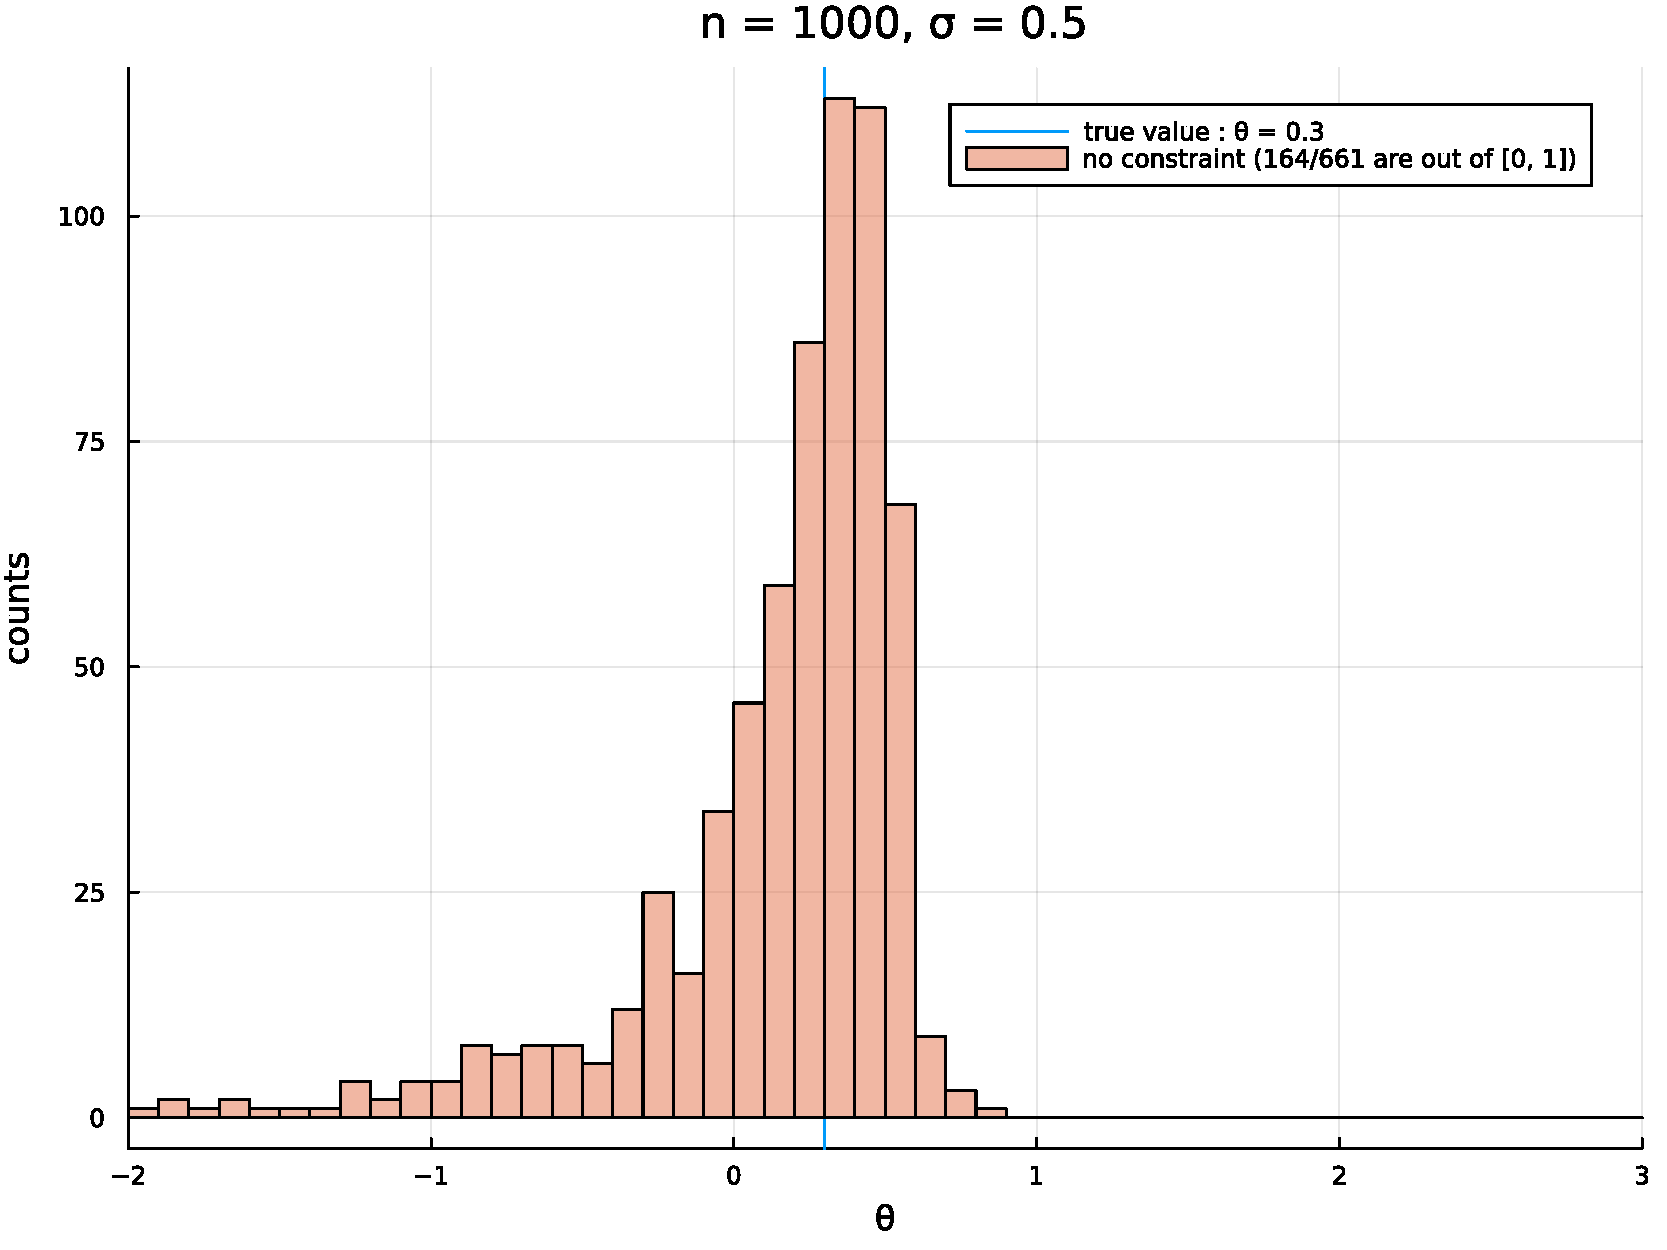
\includegraphics[width = 0.5\textwidth]
  {figuretable/histogram_loglinear_loglinear_n_1000_sigma_0.5_non_constraint.pdf}}
  \subfloat[]{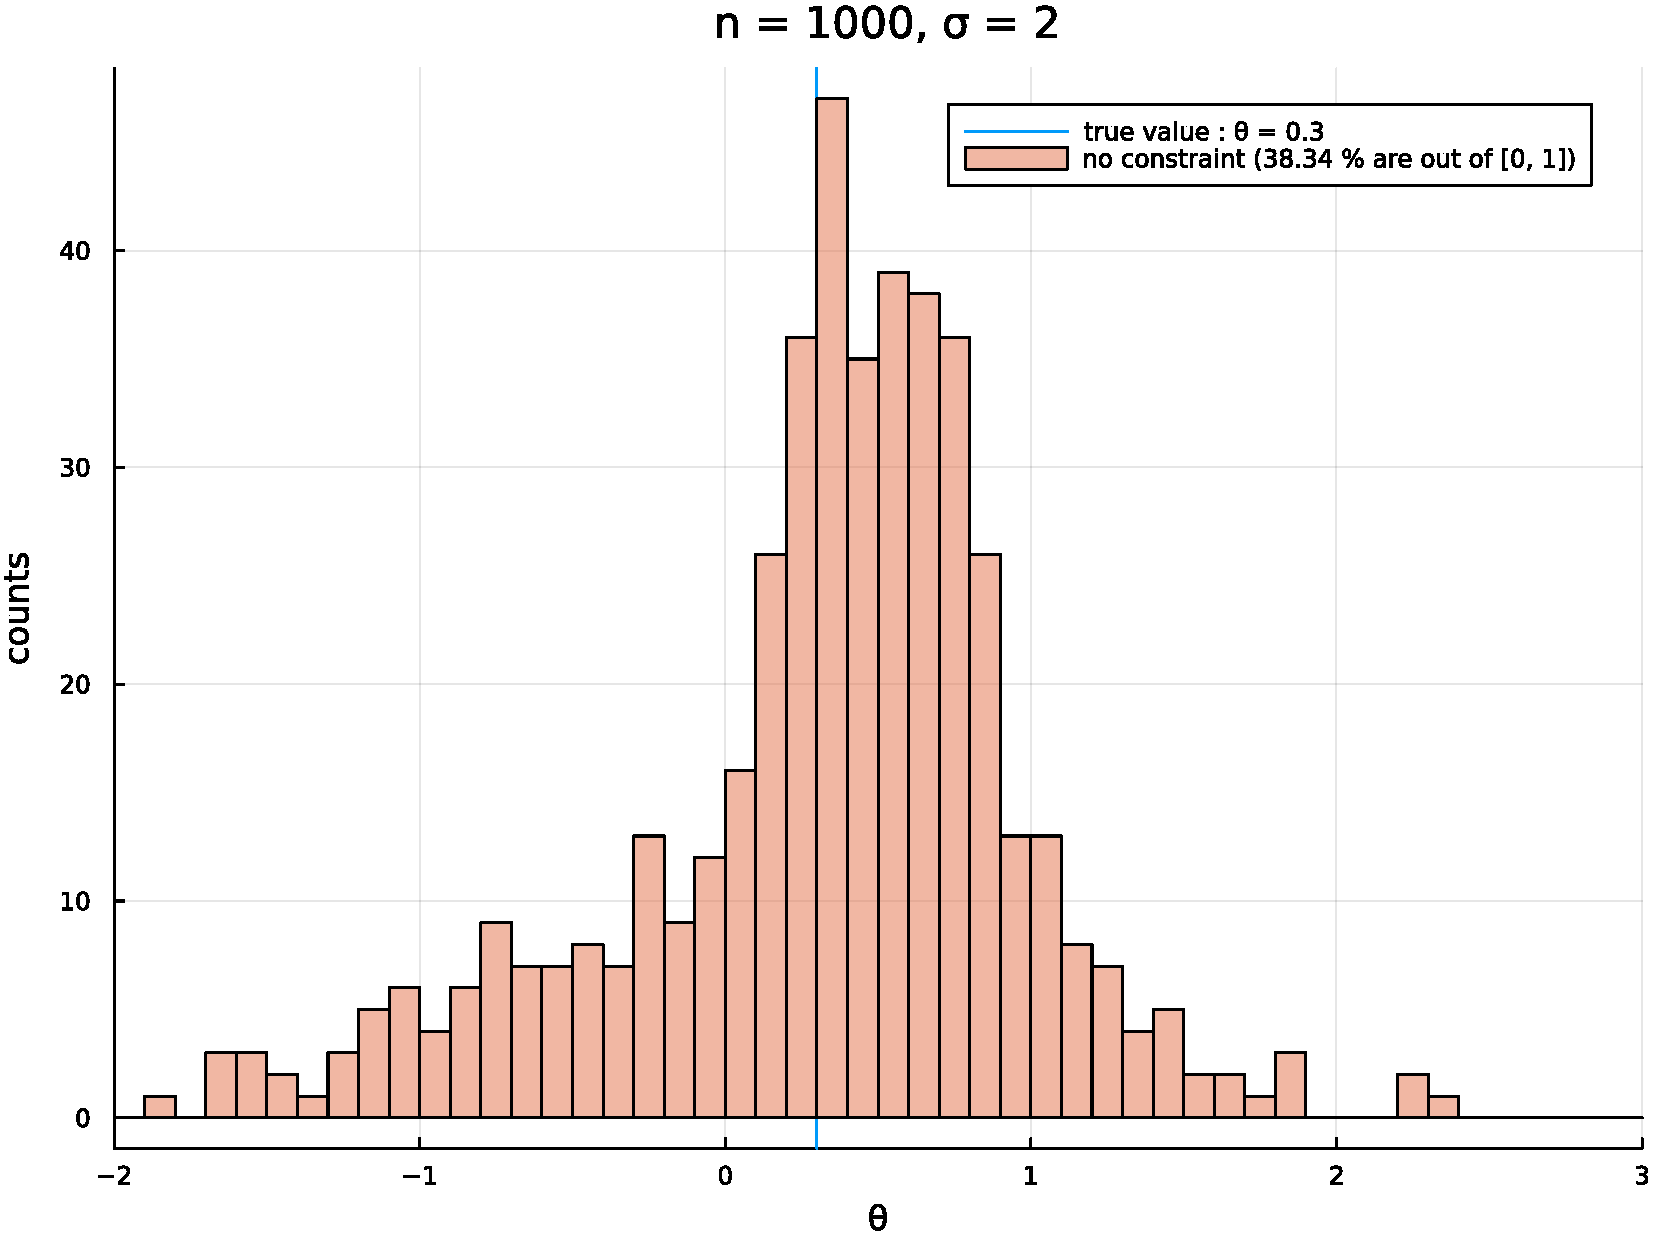
\includegraphics[width = 0.5\textwidth]
  {figuretable/histogram_loglinear_loglinear_n_1000_sigma_2_non_constraint.pdf}}
  \caption{Histograms of the estimation result of the conduct parameter.}
  \label{fg:histogram_loglinear_loglinear_no_constraint} 
  \end{center}
  \footnotesize
  Note: True parameters: $\alpha_1 = \alpha_3 = \gamma_0 = \gamma_1 = \gamma_2  = \gamma_3 = 1, \alpha_0 = 10, \alpha_2 = 0.1,  \theta = 0.3.$
\end{figure}

Why can such values arise as a solution of the GMM estimation?
To check this, for each simulation, we compute (1) the absolute differences between the true and estimated values of $\theta$ and $\gamma_0$ and (2) the absolute differences between the value of the GMM objective function under the true and estimated parameter.
Figure \ref{fg:diff_gmm_loglinear_loglinear} shows the plot of these differences. 
Each dot corresponds to each simulation and the color of each dot represents the value of the difference in the GMM objective function. 
We can see dark dots even when the difference in the conduct parameter is large.
For example, when $\sigma = 0.5$, dark dots appear when the difference is more than 10.
When $\sigma = 2.0$, dark dots appear even when the difference is more than 20.
While \citet{lau1982identifying} shows the joint identification of the conduct and cost parameter in a general case, Figure \ref{fg:diff_gmm_loglinear_loglinear} implies that the estimation becomes imprecise.


\begin{figure}[!htbp]
  \begin{center}
  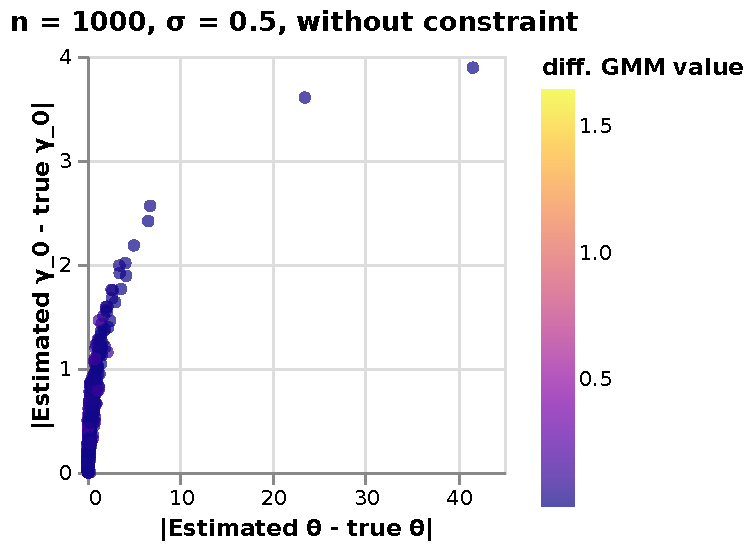
\includegraphics[width = 0.45\textwidth]
  {figuretable/diff_gmm_value_loglinear_loglinear_n_1000_sigma_0.5_non_constraint.pdf}
  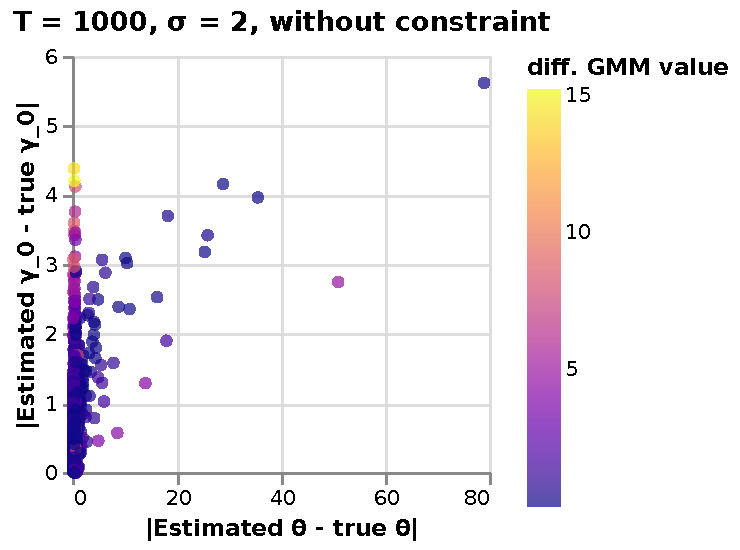
\includegraphics[width = 0.45\textwidth]
  {figuretable/diff_gmm_value_loglinear_loglinear_n_1000_sigma_2_non_constraint.pdf}
  \caption{The difference of the GMM objective function under true parameter and the estimation result}
  \label{fg:diff_gmm_loglinear_loglinear} 
  \end{center}
  \footnotesize
  Note: The x-axis is the difference between the values of the true and estimated conduct parameter. The y-axis is the difference between the values of estimated and true $\gamma_0$. Each dot represents the value of the difference of the GMM objective function under the true and estimated values of the parameters. 
\end{figure} 

%688words by Suguru


\section{Conclusion}
We revisit the conduct parameter estimation in homogeneous goods markets. In contrast to the pessimistic simulation results shown in PS, our simulation shows that the estimation becomes accurate by properly adding demand shifters in the supply estimation and increasing the sample size. We also show that the log-linear model recommended by PS has another estimation problem. Based on the numerical investigation, we conclude that at least the linear model can achieve a proper estimation of the conduct parameter in homogeneous good markets.
% 82 words

\bibliographystyle{aer}
\bibliography{conduct_parameter}

\newpage
\appendix
\section{Other experiments (Online appendix)}
\begin{table}[!htbp]
    \caption{Estimation results in Table 2 of from PS}
    \label{tb:linear_linear_sigma_Perloff_Shen}
    \begin{center}
        \begin{tabular}{cllll}
            \hline
            & $\sigma=0.001$ & $\sigma=0.5$ & $\sigma=1$ & $\sigma=2$ \\
            $\alpha_0$ & $10.00\ (0.001)$ & $9.96\ (0.33)$ & $9.86\ (0.65)$ & $9.46 (1.20)$ \\
            $\alpha_1$ & $1.00\ (0.004)$ & $0.99\ (1.98)$ & $0.97\ (3.96)$ & $0.88 (7.80)$ \\
            $\alpha_2$ & $1.00\ (0.004)$ & $0.99\ (0.21)$ & $0.97\ (0.42)$ & $0.87\ (0.82)$ \\
            $\gamma_1$ & $0.46\ (0.88)$ & $0.46\ (0.91)$ & $0.47\ (0.93)$ & $0.49\ (1.04)$ \\
            $\gamma_2$ & $5.85\ (7.89)$ & $5.85\ (8.15)$ & $5.78\ (8.21)$ & $5.73\ (8.66)$ \\
            $\theta$ & $-0.31\ (1.31)$ & $-0.29\ (1.34)$ & $0.09\ (11.48)$ & $-1.53\ (30.41)$ \\
            \hline
        \end{tabular}
    \end{center}\footnotesize
    Note: True parameters: $\alpha_1 = \alpha_2 = \gamma_0 = \gamma_1 = \gamma_2  = \gamma_3 = 1, \alpha_0 = 10, \alpha_3 = 0,  \theta = 0.5$. PS exclude $Y_t$. We change the parameter notations from the original paper. Note that PS do not provide $\gamma_0$ and $\gamma_3$.
\end{table}

First, we replicate the result in PS.
To replicate the result, we exclude the demand shifter $Y_t$ and assume the coefficient $\alpha_3$ of $Y_t$ is zeros, that is, there is no demand shifter for the supply e
For reference, Table \ref{tb:linear_linear_sigma_Perloff_Shen} is quoted from PS, although we modify some notations.
The sample size in each simulation data is 50 and the table shows the mean and the standard deviation of the 2SLS estimators from 1000 simulations.
It shows that the demand estimation becomes more accurate as the value of the standard deviation of the error terms $\sigma$ decreases.
In contrast, the supply-side estimation is still biased and the standard deviation of the conduct parameter becomes larger as the value of $\sigma$ increases.

Table \ref{tb:linear_linear_sigma_1_without_demand_shifter_y} shows our replication results.
Each panel shows the simulation result under different standard deviations of the error terms.
This result uses the same data generation process as PS. 
To see if we can correctly replicate the result in PS, focus on the first two columns in each panel.
These two columns show the mean and the standard deviation of the simulation result when the sample size is 50.
While the demand parameter can be accurately estimated even though the value of $\sigma$ becomes larger, the supply side parameter is biased.
Especially, when $\sigma$ is large and the sample size is small, the standard deviation of the parameters in the supply-side equation becomes large.
Thus, we can see the patterns in PS which do not provide any details.

As PS fix the sample size to 50, we also see the effect of changing the sample size.
As expected, increasing the sample size given a value of $\sigma$ decreases the standard deviation of the parameter in the supply equation.
However, no simulation result is close to the true values of the supply parameters and the conduct parameter.
These results are consistent with PS.

\begin{table}[!htbp]
  \begin{center}
      \caption{Estimation results of the linear model without demand shifter}
      \label{tb:linear_linear_sigma_1_without_demand_shifter_y} 
      \subfloat[$\sigma=0.001$]{
\begin{tabular}[t]{lrrrrrrrr}
\toprule
  & (1) $n=50$ / Mean & (1) $n=50$ / SD & (2) $n=100$ / Mean & (2) $n=100$ / SD & (3) $n=200$ / Mean & (3) $n=200$ / SD & (4) $n=1000$ / Mean & (4) $n=1000$ / SD\\
\midrule
$\alpha_{0}$ & 10.000 & 0.0009 & 10.000 & 0.0006 & 10.000 & 0.0004 & 10.000 & 0.0002\\
$\alpha_{1}$ & 1.000 & 0.004 & 1.000 & 0.003 & 1.000 & 0.002 & 1.000 & 0.0009\\
$\alpha_{2}$ & 1.000 & 0.0005 & 1.000 & 0.0003 & 1.000 & 0.0002 & 1.000 & 0.0001\\
$\gamma_{0}$ & 5.446 & 6.981 & 5.388 & 7.986 & 5.423 & 7.825 & 5.063 & 6.801\\
$\gamma_{1}$ & 0.506 & 0.775 & 0.512 & 0.888 & 0.509 & 0.869 & 0.549 & 0.756\\
$\gamma_{2}$ & 0.506 & 0.776 & 0.512 & 0.887 & 0.509 & 0.869 & 0.549 & 0.756\\
$\theta$ & -0.241 & 1.164 & -0.231 & 1.331 & -0.237 & 1.304 & -0.177 & 1.134\\
$R^{2}$ (demand) & 1.000 & 0.0000004 & 1.000 & 0.0000003 & 1.000 & 0.0000002 & 1.000 & 8e-08\\
$R^{2}$ (supply) & 1.000 & 0.000008 & 1.000 & 0.00001 & 1.000 & 0.00001 & 1.000 & 0.000008\\
Sample size ($T$) &  & 50 &  & 100 &  & 200 &  & 1000\\
\bottomrule
\end{tabular}
}\\
      \subfloat[$\sigma=0.5$]{
\begin{tabular}[t]{lrrrrrrrr}
\toprule
  & (1) $n=50$ / Mean & (1) $n=50$ / SD & (2) $n=100$ / Mean & (2) $n=100$ / SD & (3) $n=200$ / Mean & (3) $n=200$ / SD & (4) $n=1000$ / Mean & (4) $n=1000$ / SD\\
\midrule
$\alpha_{0}$ & 9.993 & 0.466 & 9.993 & 0.312 & 10.001 & 0.215 & 10.002 & 0.093\\
$\alpha_{1}$ & 0.963 & 2.138 & 0.965 & 1.484 & 1.012 & 1.023 & 0.991 & 0.441\\
$\alpha_{2}$ & 1.002 & 0.243 & 1.002 & 0.168 & 0.999 & 0.118 & 1.002 & 0.049\\
$\gamma_{0}$ & 5.332 & 10.459 & 5.227 & 11.592 & 5.112 & 15.871 & 5.470 & 7.476\\
$\gamma_{1}$ & 0.405 & 3.214 & 0.434 & 1.989 & 0.474 & 1.744 & 0.516 & 1.102\\
$\gamma_{2}$ & 0.517 & 1.157 & 0.528 & 1.222 & 0.546 & 1.816 & 0.504 & 0.830\\
$\theta$ & -0.210 & 1.879 & -0.206 & 1.951 & -0.186 & 2.705 & -0.247 & 1.238\\
$R^{2}$ (demand) & 0.720 & 0.088 & 0.725 & 0.061 & 0.726 & 0.041 & 0.728 & 0.018\\
$R^{2}$ (supply) & 0.160 & 7.674 & -0.119 & 19.529 & -0.724 & 30.775 & 0.491 & 2.041\\
Sample size (n) &  & 50 &  & 100 &  & 200 &  & 1000\\
\bottomrule
\end{tabular}
}\\
  \end{center}\footnotesize
  Note: True parameters: $\alpha_1 = \alpha_2 =  \gamma_0 = \gamma_1 = \gamma_2  =  1, \alpha_0 = 10, \theta = 0.5.$ and $\alpha_3 =0$
\end{table} 

\begin{table}[!htbp]
  \ContinuedFloat
  \begin{center}
      \caption{Estimation results of the linear model without demand shifter (Continued)}
      \subfloat[$\sigma=1.0$]{
\begin{tabular}[t]{lrrrrrrrr}
\toprule
  & Mean & SD & Mean  & SD  & Mean   & SD   & Mean    & SD   \\
\midrule
$\alpha_{0}$ & 9.975 & 0.964 & 9.953 & 0.636 & 10.007 & 0.441 & 9.991 & 0.189\\
$\alpha_{1}$ & 1.120 & 4.491 & 0.942 & 2.885 & 0.883 & 2.055 & 1.035 & 0.902\\
$\alpha_{2}$ & 0.981 & 0.492 & 0.993 & 0.326 & 1.015 & 0.227 & 0.993 & 0.101\\
$\gamma_{0}$ & 5.631 & 9.410 & 5.520 & 7.580 & 5.161 & 9.226 & 5.556 & 7.424\\
$\gamma_{1}$ & -0.107 & 19.285 & 0.129 & 5.240 & 0.488 & 3.541 & 0.489 & 1.210\\
$\gamma_{2}$ & 0.476 & 1.043 & 0.495 & 0.835 & 0.540 & 1.030 & 0.494 & 0.820\\
$\theta$ & -0.201 & 3.603 & -0.217 & 1.478 & -0.183 & 1.528 & -0.260 & 1.229\\
$R^{2}$ (demand) & 0.205 & 0.357 & 0.234 & 0.221 & 0.232 & 0.150 & 0.245 & 0.060\\
$R^{2}$ (supply) & -0.920 & 17.898 & -0.395 & 5.271 & -0.904 & 12.486 & -0.421 & 12.047\\
Sample size (n) &  & 50 &  & 100 &  & 200 &  & 1000\\
\bottomrule
\end{tabular}
}\\
    \subfloat[$\sigma=2.0$]{
\begin{tabular}[t]{lrrrrrrrr}
\toprule
  & Mean & SD & Mean  & SD  & Mean   & SD   & Mean    & SD   \\
\midrule
$\alpha_{0}$ & 9.515 & 6.752 & 9.912 & 1.479 & 9.987 & 0.943 & 9.987 & 0.396\\
$\alpha_{1}$ & 0.362 & 19.344 & 0.710 & 6.192 & 1.154 & 4.363 & 0.986 & 1.728\\
$\alpha_{2}$ & 0.934 & 1.092 & 1.004 & 0.743 & 0.981 & 0.494 & 0.998 & 0.204\\
$\gamma_{0}$ & 5.658 & 6.892 & 5.464 & 8.387 & 5.695 & 8.243 & 5.572 & 10.796\\
$\gamma_{1}$ & 0.956 & 52.166 & 1.715 & 42.062 & -0.056 & 11.467 & 0.388 & 3.140\\
$\gamma_{2}$ & 0.479 & 0.827 & 0.496 & 0.907 & 0.486 & 0.902 & 0.497 & 1.185\\
$\theta$ & -0.296 & 5.941 & -0.439 & 5.106 & -0.235 & 2.034 & -0.256 & 1.771\\
$R^{2}$ (demand) & -3.456 & 87.362 & -0.513 & 1.557 & -0.436 & 0.563 & -0.376 & 0.185\\
$R^{2}$ (supply) & -1.104 & 5.881 & -2.311 & 26.606 & -1.993 & 26.973 & -3.591 & 49.060\\
Sample size ($T$) &  & 50 &  & 100 &  & 200 &  & 1000\\
\bottomrule
\end{tabular}
}
  \end{center}\footnotesize
  Note: True parameters: $\alpha_1 = \alpha_2 =  \gamma_0 = \gamma_1 = \gamma_2  =  1, \alpha_0 = 10, \theta = 0.5.$ and $\alpha_3 =0$
\end{table} 

\begin{figure}[!htbp]
  \begin{center}
  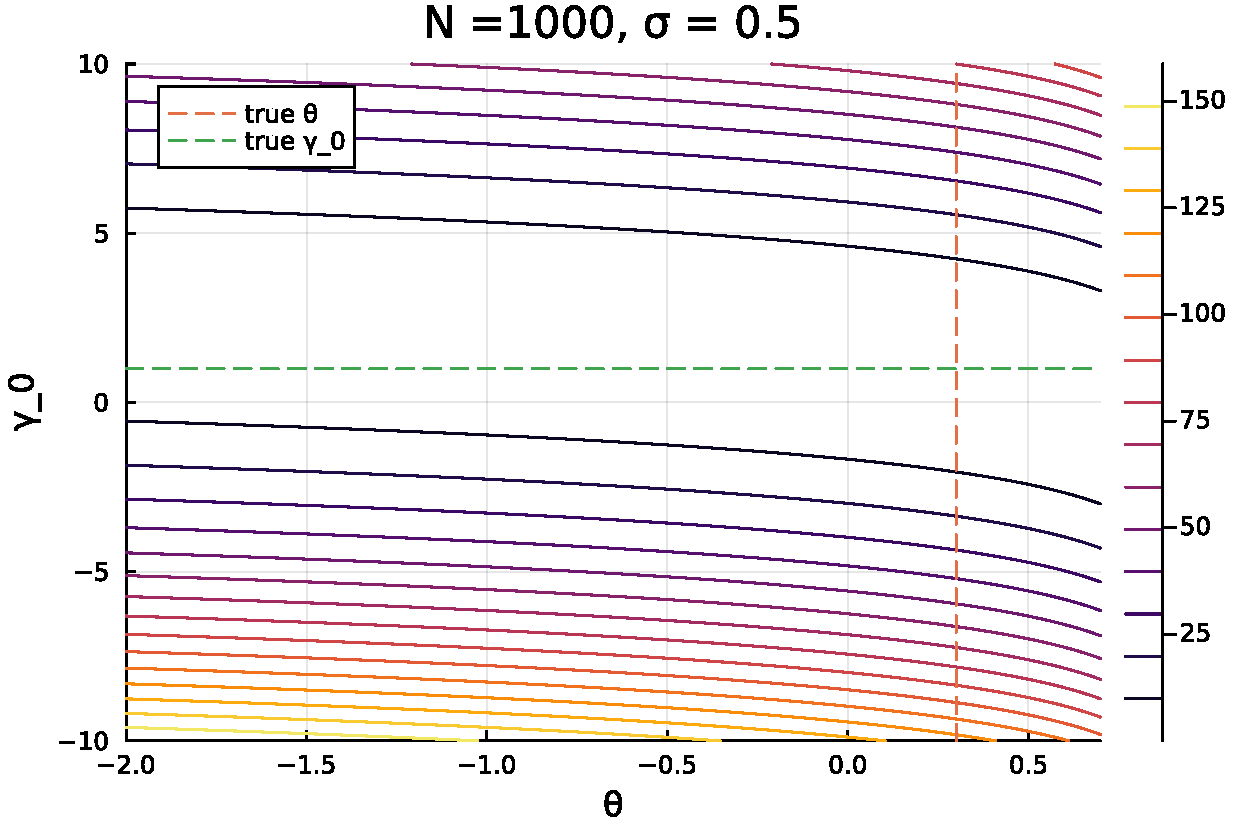
\includegraphics[width = 0.45\textwidth]
  {figuretable/contour_loglinear_loglinear_n_1000_sigma_0.5.pdf}
  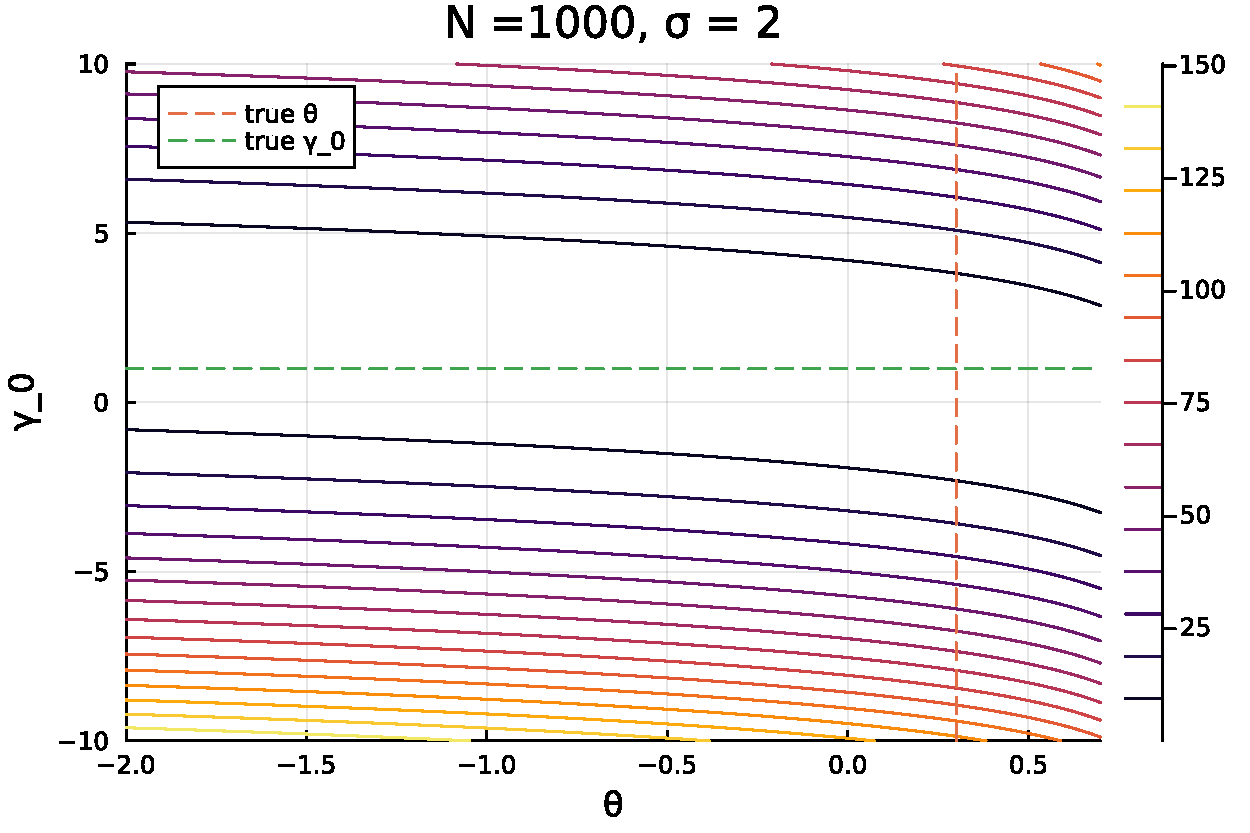
\includegraphics[width = 0.45\textwidth]
  {figuretable/contour_loglinear_loglinear_n_1000_sigma_2.pdf}
  \caption{Contour map of GMM objective function}
  \label{fg:contour_loglinear_loglinear_n_1000_sigma_2} 
  \end{center}
  \footnotesize
  Note: True parameters: $\alpha_1 = \alpha_3 = \gamma_0 = \gamma_1 = \gamma_2  = \gamma_3 = 1, \alpha_0 = 10, \alpha_2 = 0.1,  \theta = 0.3.$
\end{figure} 

Figure \ref{fg:contour_loglinear_loglinear_n_1000_sigma_2} illustrates the contour map of the GMM objective function with respect to $\gamma_0$ and $\theta$ for one typical data.
To draw the map, we fix the other demand and cost parameter values to the true values and set the grid size to 0.01.
We can see that the contour map has a flat region around the true parameters.
Especially, even though we vary the value of $\theta$, the GMM value does not change around the true value of $\gamma_0$.

First, note that in Table \ref{tb:loglinear_loglinear_non_constraint}, the mean of $\gamma_0$, the constant term in the log-linear marginal cost function, is far from the true parameter and the standard deviation is large compared with other marginal cost parameters. 
Recall that the first and second term in the supply equation \eqref{eq:log_linear_supply_equation} is $-\log(1 - \theta(\alpha_1 + \alpha_2 Z^{R}_{t})) + \gamma_0$.
As the first term is always negative, for any value of $\theta$ that satisfies $1 - \theta(\alpha_1 + \alpha_2 Z^{R}_{t})$, we can find a value of $\gamma_0$ that cancel out the first and the second term each other.
Especially when the other estimated parameters are close to the true value, by adjusting the value of $\theta$ and $\gamma_0$ to cancel out the first and second term, we can make the value of the GMM objective function under the estimated parameters close to the value of the GMM objective function under the true parameter.


\end{document}